\section{Implementation Concepts}
\label{sec:eventdriven_implementation}

TODO WEAK CHAPTER TOO AD-HOC, CAN BE DONE MUCH BETTER BOTH AT EXPLAINING AND CONTENT, NEEDS REFACTORING
- motivate each step carefully step-by-step, ultimately we derive immutable, pure functional objects here which we became aware of only after we properly reflected on it in the conclusions. this is no coincidence: the deeper idea behind objects (exchange of messages with shared nothing semantics with internal immutable state) seems indeed to be a good approach to ABS. indeed, we could also implement a sugarscape completely different with pure functions and data-structures over which we iterate: this is then a completely data-centric approach without any encapsulation and abstraction: this is what we do NOT want here, TODO: why not? encapsulation and abstraction is good, otherwise we have a blob of mutable data with a data-flow which is difficult to reason about, even if it is pure functional programming. In ACE this is less a problem, as the gintis case and the zero intelligence implementations show: agents there can be really implemented using a simple newtype or data-structures with pure functions (and a few MonadRandom ones), why? because there the model is much more about data, data-representation and data-flow than interaction of agents like in the sugarscape.
This is also a bit the case in the previous chapter on time-driven ABS where the agents act continously over time, reflecting a much more data-flow centric approach than an interaction-centric one. In this chapter the interaction move into the center and we show how to achieve that in ABS: how we can represent interacting agents in a pure functional way. The reason why we named it event-driven is that events or messages are the heart of interactions between agents; after all it is no coincidence that in OO terminology method calls are also synonymous with sending a message to an object
- can we follow a cleaner Tagless Final approach like i prototyped in SIR? this allows easier extensibility in both dimensions: adding new operations (what agents are allowed to do) and new interpreter (pure functional, STM concurrency, IO concurrency). I will learn a great deal about this, it will be a strong selling point and it might event allow to implement synchronous interactions?? 
- use MTL instead of fully expanded stack! e.g. MonadRandom instead of Rand
% https://jproyo.github.io/posts/2019-03-17-tagless-final-haskell.html
% https://serokell.io/blog/2018/12/07/tagless-final
- In the time-driven approach we already introduced the use of effectful SignalFunctions: Monadic Stream Functions (MSF), where we only used a simple Rand effect to draw random number streams. Due to the much greater complexity of the Sugarscape we will want to make use of a whole layer of effects. To manage them in a clean way we follow a so called \textit{Tagess Final} approach \cite{kiselyov_typed_2012}. The idea relies heavily on defining operations using type-classes and the implementing concrete instances for them which act as interpreters. The main benefit is that a Tagless Final approach is extensible in two dimensions according to the Extension Problem (TODO: cite the paper): we can add new interpreters to existing data-types (TODO what part of the extension problem is that) and we can add new operations (TODO: what part of the extension problem is that?). Ultimately, this allows us to separate specification from implementation, following a similar approach as Free Monads (see future research) without the problems of their performance penalty.


TODO REFINE CONTENT: we can write combinators which encapsulate all the continuation plumbing so it looks in the end very similar to a method call: shortly discuss and show that in Sugarscape. implement sync-interaction combinator: it becomes clear in the type of the function what is going on

In the next sections we derive implementation concepts of pure functional event-driven ABS. Due to the complexity of the Sugarscape model we don't provide a full implementation but only present concepts derived from our implementation and present small parts of the Sugarscape implementation when necessary.

\subsection{Agent Representation}
We follow the same approach as in the time-driven approach of Chapter \ref{sec:timedriven_monadic} and use an MSF to define our agent due to the following requirements:

\begin{itemize}
	\item As in the time-driven approach, we need a random number stream within our agents, for which we will make use of the \textit{Rand} monad.
	
	\item In the Sugarscape, the agents act on an environment which they both read \textit{and} write. We will make use of the \textit{State} monad for this functionality. 
	
	\item The agents state in the Sugarscape model is much more complex than in the time-driven example where it was implicit. In this approach the agents have an explicit data-structure which they can mutate whenever they are acting. We will make use of the \textit{State} monad for this functionality.
	
	\item For synchronous and one-way agent-interactions, agents send messages to other agents. This is completely different from the time-driven approach where no direct agent-interactions in form of messages where possible because agents were all acting at the same time and synchronous agent-interactions would violate that principle. We will make use of the \textit{Writer} monad for this functionality.

	\item Due to the agent-interaction through messaging we need a clearly defined concept of agent identity, which is immutable for each agent and fixed at agent-creation time. At the same time we also need to generate new agent identities e.g. when an agent needs to create a new born from mating action. Further we need to access the read-only model configuration which defines if e.g. trading is turned on or off. We will make use of the \textit{Reader} and \textit{State} monad for this functionality.
\end{itemize}

The interface of an agent changes now substantially with very different inputs and outputs due to the fundamental different model and ABS type. Because we are dealing with events now, it makes very much sense to define the input-type of an agent as the event-type: this indicates that an agent always needs an event to run, to which it will react. As output we need a much richer structure than simply the current state the agent is in as in the time-driven approach: we need to be able to communicate to the simulation kernel whether the agent should be removed from the simulation, what new agents this agent wants to create and what messages it sends to other agents. Additionally we need to communicate the observable properties of an agent to the simulation kernel for visualisation purposes. We will show below how to conveniently construct such an output in a monadic way through the \textit{Writer} monad. Note that many additional inputs and outputs are implicitly covered by the monadic context as will be shown below, e.g. we could also pass the environment as input and returning it as output instead providing it through a \textit{State} monad but the latter is much more convenient to program with.

\subsubsection{A generic MSF for event-driven ABS}
We start with defining the basic types for a general event-driven agent. Besides the obligatory Time and $\Delta t$ which are defined in this case as \textit{Int} we define an \textit{AgentId} as \textit{Integer} for uniquely identifying agents in the process of messaging. Further an event type is defined which is either a \textit{Tick} with a given $\Delta t$ or a \textit{DomainEvent} from a given sender with the given event where the type of the actual \textit{DomainEvent} is generic. As already mentioned we need a way of generating new agent identities which happens through the \textit{ABSState} data structure which holds the next agent-id plus the current virtual simulation time so that agents don't need to keep track of it themselves. Now we can define the initial \textit{AgentT} monad-transformer for which we start with a \textit{StateT} and the previously defined \textit{ABSState}. 

Finally we define the type of the Agent MSF as a simple monadic stream function (MSF) with the monadic context \textit{AgentT} and the \textit{ABSEvent} as input. The output is the previously mentioned structure and the observable properties of the agent. The Agent MSF is parametrised by \textit{m} indicating the type of (additional) monadic context, \textit{e} indicating the type of the \textit{DomainEvent} and \textit{o} indicating the type of the observable properties. These types are highly polymorphic and are applicable to a wide range of event-driven ABS models. Note that no explicit type of an environment is used because some models rather omit an explicit environment and have it implicitly encoded in the model itself e.g. a fully connected network of agent-neighbourhoods as in the agent-based SIR model in Chapter \ref{sec:timedriven_firststep}. Further, we also don't provide random-number generator functionality on the type-level at that point because concrete models might opt for a different approach to randomness e.g. providing their own random number generator through a monad-transformer or omitting it altogether. All this optional behaviour is possible because the monadic context of the agents MSF is a transformer which allows to add arbitrary number of layers of behaviour as we will see below: we are polymorphic in the side-effects, which is only possible in a pure functional language like Haskell and can't be achieved in the established OOP approaches to ABS.

\begin{HaskellCode}
type Time  = Int
type DTime = Int

type AgentId = Integer

data ABSEvent e = Tick DTime | DomainEvent AgentId e
                
data ABSState = ABSState
  { absNextId :: AgentId -- holds the next agent-id 
  , absTime   :: Time    -- current simulation time
  }

type AgentT m       = StateT ABSState m
type AgentMSF m e o = MSF (AgentT m) (ABSEvent e) (AgentOut m e o, o)

-- definition of a new agent 
data AgentDef m e o = AgentDef
  { adId      :: AgentId         -- unique agent-id
  , adSf      :: AgentMSF m e o  -- the agent behaviour function
  , adInitObs :: o               -- the value of the initial observable properties
  }

data AgentOut m e o = AgentOut 
  { aoKill   :: Any              -- True if this agent should be removed 
  , aoCreate :: [AgentDef m e o] -- a list of agents to create
  , aoEvents :: [(AgentId, e)]   -- a list of events (receiver, event)
  }
\end{HaskellCode}

What is striking, and underlines the even-driven approach, is that we are using an MSF and not a monadic SF (Streamfunction) from Bearriver as we did in Chapter \ref{sec:timedriven_monadic}. This means that there is no inherent notion of a $\Delta t$ available to the agent, which is precisely what we need in event-driven ABS. Time only advances through specific events, in this case the \textit{Tick DTime} event.

\subsubsection{Parametrising for Sugarscape}
For our Sugarscape implementation, we need to parametrise the polymorphic types by concrete types for \textit{m}, \textit{e} and \textit{o}. Further, we need access to a random-number stream and we want to make the unique agent-id, the environment and the model-configuration explicit in the types. We start with defining both the environment and model-configurations as new data-structures (see below) and the data-type for an individual agent-state and the observable properties of the agent. Note that we explicitly decided to use two different types for the agent-state and its observable properties - after all we could have used the type of the agent-state also as the type for its observable properties. With two different types we make the distinction between the (read/write) local agent-state and the (read-only) observable properties very clear. Also, it allows us to expose a much smaller subset of the agent-local state to the visualisation and export layer of the simulation. This gives us the ability to hide away agent-state fields, which are implementation detail or unimportant for visualisation and exporting purposes.

\begin{HaskellCode}
data SugEnvironment     = ...
data SugarScapeScenario = ...

data SugAgentState = SugAgentState
  { sugAgSugarMetab   :: Int
  , sugAgVision       :: Int
  , sugAgSugarLevel   :: Double
  , sugAgInitSugEndow :: Double
  , sugAgAge          :: Int
  , ...
  }
  
data SugAgentObservable = SugAgentObservable
  { sugObsSugMetab :: Int
  , sugObsVision   :: Int
  , sugObsSugLvl   :: Double
  , sugObsAge      :: Int
  ...  
  }
\end{HaskellCode}

As already mentioned, we can add additional behaviour through the monad transformer of the agents MSF. We use this to make the Sugarscape environment explicit in the types and add random number-functionality. We simply start out with a \textit{StateT} transformer for the Sugarscape environment, because the agent can read and write it and then terminate the transformer by adding the \textit{Rand} monad for the random-number functionality. We then simply parametrise the existing monad transformer of \textit{AgentMSF} with this additional transformer stack to arrive at the final type of the Sugarscapes agent MSF.

\begin{HaskellCode}
data SugEvent = ... -- all events of the sugarscape model

type SugAgentMonad g = StateT SugEnvironment (Rand g)
-- the sugarscape agent MSF with the monadic type expanding to:
-- AgentMSF (SugAgentMonad g)
-- => 
-- MSF (AgentT (SugAgentMonad g))
-- => 
-- MSF (StateT ABSState (SugAgentMonad g))
-- =>
-- MSF (StateT ABSState (StateT SugEnvironment (Rand g)))
type SugAgentMSF g = AgentMSF (SugAgentMonad g) SugEvent SugAgentObservable
\end{HaskellCode}

Finally we define the type of the top-level agent-behaviour function. As already noted, we want to make the unique agent-id and the model-configuration explicit, so it will be passed as an argument to the function. Further we pass the initial agent state as an additional input. This function will then construct a corresponding initial MSF (see below) and returns it. Thus the intended behaviour is as follows: an agent is defined in terms of this top-level function, which will be passed to the simulation kernel (see below) which will in turn run this function to get the agents initial MSF which will then be run subsequently (see below).

\begin{HaskellCode}
type SugarScapeAgent g = SugarScapeScenario -> AgentId -> SugAgentState -> SugAgentMSF g
\end{HaskellCode}

Now we have fully specified types for the Sugarscape agent. The types indicate very clearly the intention and the interface. What is of very importance is that we don't have any impure \textit{IO} monadic context anywhere in our type-definitions and we can also guarantee that it won't get sneaked in: the transformer-stack of the agents MSF is terminated through the \textit{Rand} monad - it is simply not possible to add other layers. In the next step we look at how the agent handles and send events - that is we are looking at an implementation of a \textit{SugarScapeAgent} function.

\subsubsection{Agent-Local abstractions}
The top-level \textit{SugarScapeAgent} function encapsulates the whole agent-behaviour, which is completely driven by events, passed in as input. We now look at how to define agent-local behaviour, which is hidden behind the \textit{SugarScapeAgent} function-type: whereas the previously defined types are exposed to the whole simulation, the following deals with types and behaviour which is locally encapsulated and hidden from the simulation kernel. We want to achieve the following functionality, local to the agent: encapsulation of the agents' state which should still be read/writeable, sending of events and read-only access to the agents unique id and the model configuration.

To implement the local encapsulation of the agents' state is straight forward with MSFs as they are continuations, which allow to capture local data using closures. Fortunately we don't need to implement the low-level plumbing, as dunai provides us with the a feedback function: \textit{feedback :: Monad m $\Rightarrow$ c $\rightarrow$ MSF m (a, c) (b, c) $\rightarrow$ MSF m a b}. It takes an initial value of type \textit{c} and an MSF which takes in addition to its input \textit{a} also the given type \textit{c} and outputs in addition to type \textit{b} also the type \textit{c}, which clearly indicates the read/write property of type \textit{c}. The function returns a new MSF which only operates on \textit{a} as input and returns \textit{b} as output by running the provided MSF and feeding back the \textit{c} (with the initial \textit{c} at the first call).

\begin{HaskellCode}
agentMsf :: RandomGen g => SugarScapeAgent g
agentMsf params aid s0 = feedback s0 (proc (evt, s) -> do ... )
\end{HaskellCode}

Next we want to write a monadic function which handles our event. As already pointed out this function must be able to manipulate the agent-local state we just encapsulated through \textit{feedback}, sending events and accessing the model configuration and the unique agent-id. Providing the local agent state is trivially done using the \textit{State} monad. Providing the model configuration and the unique agent-id is trivially done using the \textit{Reader} monad. For providing the event sending function we opted for the \textit{Writer} monad: as shown above in the generic types, an agent outputs (amongst others) a list of events it wants to send to receivers. Thus we start with an empty initial list and provide functionality to append to this list - which is exactly what the \textit{Writer} monad does: it allows to write to a data-type which implements the \textit{Monoid} class. The lists in Haskell are instances of the \textit{Monoid} class, thus this is covered for us already. Instead of only covering the event sending functionality with the \textit{Writer} monad, we extend it to the whole \textit{SugAgentOut} type which respective fields are instances of the \textit{Monoid} class themselves thus writing an instance of the \textit{Monoid} class for \textit{SugAgentOut} is trivial. We thus define the following monad which is local to the agent and is only used \textit{within} \textit{AgentMSF}.

\begin{HaskellCode}
type SugAgentMonadT g = AgentT (SugAgentMonad g)
-- FULLY EXPANDS TO:
-- AgentT (SugAgentMonad g)
--  =>
-- AgentT (StateT SugEnvironment (Rand g))
--  =>
-- StateT ABSState (StateT SugEnvironment (Rand g))

type AgentLocalMonad g = WriterT (SugAgentOut g) 
                           (ReaderT (SugarScapeScenario, AgentId) 
                             (StateT SugAgentState (SugAgentMonadT g)))
-- FULLY EXPANDS TO (one step replacement of SugAgentMonadT):
-- WriterT (SugAgentOut g) 
--  (ReaderT (SugarScapeScenario, AgentId) 
--    (StateT SugAgentState 
--      (StateT ABSState 
--        (StateT SugEnvironment 
--          (Rand g)))  
\end{HaskellCode}

Now we can define the MSF which handles an event. It has the \textit{AgentLocalMonad} monadic context, takes an \textit{ABSEvent} parametrised over \textit{SugEvent} (thus it has also to handle \textit{Tick}). What might come as a surprise is that it returns unit-type, implying that the results of handling an event are only visible as side-effects in the monad stack. This is intended. We could pass all arguments explicitly as input and/or output but that would complicate the handling code substantially, thus we opted for a monadic, imperative style handling of events.

\begin{HaskellCode}
type EventHandler g = MSF (AgentLocalMonad g) (ABSEvent SugEvent) ()
\end{HaskellCode}

To run the handler, which has an extended monadic context within the \textit{SugarScapeAgent} we make use of dunais functionality which provides functions to run MSFs with additional monadic layers within MSFs with less - similar to the \textit{Control.Monad} approach. We use \textit{runStateS}, \textit{runReaderS} and \textit{runWriterS} (\textit{S} indicates the stream character) to run the \textit{generalEventHandler}, providing the initial values for the respective monads: \textit{s} for the \textit{StateT}, \textit{(params, aid)} for the \textit{ReaderT} and the \textit{evt} as the normal input to the event handler. Note that \textit{WriterT} does not need an initial value, it will be provided through the \textit{Monoid} instance of \textit{AgentOut}.

\begin{HaskellCode}
agentMsf :: RandomGen g => SugarScapeAgent g
agentMsf params aid s0 = feedback s0 (proc (evt, s) -> do
  (s', (ao', _)) <- runStateS (runReaderS (runWriterS generalEventHandler)) -< (s, ((params, aid), evt))
  let obs = sugObservableFromState s
  returnA -< ((ao', obs), s'))

generalEventHandler :: RandomGen g => EventHandler g

sugObservableFromState :: SugAgentState -> SugAgentObservable
\end{HaskellCode}

\subsubsection{Handling and sending of Events}
Now we can handle events on an agent-local level: we receive the events from the simulation kernel as input and run within a 6-layered monad transformer stack which is part global to the agent (controlled by the simulation kernel) and part local to the agent (controlled by the agent itself). The layers are the following (outer to inner):

\begin{enumerate}
	\item WriterT (SugAgentOut g): \textit{agent-local}, provides write-only functionality for constructing the agent-output for the simulation kernel which indicates whether to kill the agent, a list of new agents to create and a list of events to send to receiving agents.
	\item ReaderT (SugarScapeScenario, AgentId): \textit{agent-local}, provides the model configuration and unique agent-id read-only.
	\item StateT SugAgentState: \textit{agent-local}, provides the local agent state for reading and writing.
	\item StateT ABSState: \textit{global}, provides unique agent-ids for new agents and the current simulation time. The usage of a \textit{StateT} is slightly flawed here because it provides too much power: the current simulation time should be read-only to the agent. Drawing the next agent-id involves reading the current id and writing the incremented value, thus technically it is a \textit{StateT} but ideally we would like to hide the writing operation and only provide a \textit{read-current-and-increment} operation. A possible solution would be to provide the current simulation time through a \textit{ReaderT} and the new agent-id through a new monad which uses the \textit{StateT} under the hood, like the \textit{Rand} monad.
	\item StateT SugEnvironment: \textit{global}, provides the sugarscape environment which the agents can read and write.
	\item Rand g: \textit{global}, provides the random-number stream for all agents.
\end{enumerate}

The event handler simply matches on the incoming events, extracts data and dispatches to respective handlers. What is crucial here to understand is that only the top level \textit{agentMSF} and the \textit{EventHandler} function are MSFs which simply dispatch to monadic functions, implementing the functionality in an imperative programming style. The main benefit of the MSFs are their continuation character, which allows to encapsulate local state. Further the dunai library adds a lot of additional functionality of composing MSFs and running different monadic context on top of each other. It even provides exception handling through MSFs with the \textit{Maybe} type, thus programming with exceptions in ABS models can be done as well (we didn't make use of it, as the Sugarscape model simply does not specify any exception handling on the model level and there was also no opportunity to use exceptions from which to recover on a technical level - there are exceptions on a technical level but they are non-recoverable and should never occur at runtime, thus \textit{error} is used, which terminates the simulation with an error message).

\begin{HaskellCode}
data SugEvent = MatingRequest AgentGender
              | MatingReply (Maybe (Double, Double, Int, Int, CultureTag, ImmuneSystem))
              ...
              
generalEventHandler :: RandomGen g => EventHandler g
generalEventHandler =
  continueWithAfter -- optionally switching the top event handler 
    (proc evt -> 
      case evt of 
        Tick dt -> do
          mhdl <- arrM handleTick -< dt
          returnA -< ((), mhdl)

        (DomainEvent sender (MatingRequest otherGender)) -> do
          arrM (uncurry handleMatingRequest) -< (sender, otherGender)
          returnA -< ((), Nothing)
        ...)
        
handleTick :: RandomGen g => DTime -> AgentLocalMonad g (Maybe (EventHandler g))
handleMatingRequest :: AgentId -> AgentGender -> AgentLocalMonad g ()
\end{HaskellCode}

Note the use of \textit{continueWithAfter}, which is a customised version of the already known \textit{switch} combinator, as used in Chapter \ref{sec:timedriven_firststep}. It allows to swap out the event-handler for a different one, which is the foundation for the synchronous agent-interactions, where it will be discussed more in-depth.

To see how an event handler works, we provide the implementation of \textit{handleMatingRequest}. It is sent by an agent to its neighbours to request whether they want to mate with this agent. The handler receives the sender and the other agents gender (see \textit{generalEventHandler}) and replies with \textit{sendEventTo} which sends a \textit{MatingReply} event back to the sender. The function \textit{sendEventTo} operates on the \textit{WriterT} to append (using \textit{tell}) an event to the list of events this agent sends when handling this event. Note the use of \textit{agentProperty}, which reads the value of a given field of the local agent state. 

\begin{HaskellCode}
handleMatingRequest :: AgentId
                    -> AgentGender
                    -> AgentLocalMonad g ()
handleMatingRequest sender otherGender = do
  -- check if the agent is able to accept the mating request: 
  -- fertile, wealthy enough, different gender
  accept <- acceptMatingRequest otherGender

  -- each parent provides half of its sugar-endowment for the new-born child
  acc <- if not accept
      then return Nothing
      else do
        sugLvl  <- agentProperty sugAgSugarLevel
        spiLvl  <- agentProperty sugAgSpiceLevel
        metab   <- agentProperty sugAgSugarMetab
        vision  <- agentProperty sugAgVision
        culTag  <- agentProperty sugAgCultureTag
        imSysGe <- agentProperty sugAgImSysGeno

        return Just (sugLvl / 2, spiLvl / 2, metab, vision, culTag, imSysGe)

  sendEventTo sender (MatingReply acc)
\end{HaskellCode}

Next we look at how synchronous agent-interactions work - that is we look closer at the mating-mechanism which requires multiple synchronous interaction steps, which need to happen within the same simulation tick and both agents must not engage with other agents.

\subsubsection{Synchronous Agent-Interactions}
With the concepts introduced so far we can achieve already a lot in terms of agent-interactions: agents can react to incoming events, which are either the Tick-event advancing simulation time by one step or a message sent by another agent (or the agent itself). This is enough to implement simple one-directional asynchronous agent-interactions where one agent sends a message to another agent but does not await an answer within the same tick. This one-directional asynchronous interactions is used in the model to implement the passing of diseases, the paying back of debt, passing on wealth to children upon death - the agent simply sends a message and forgets about it.

Unfortunately this mechanism is not enough to implement the other agent-interactions in the Sugarscape model, which are structurally richer: they need to be synchronous. In the use-cases of mating, trading and lending two agents need to come to an agreement over multiple interactions steps within the same tick which need to be exclusive and synchronous.  This means that an agent A initiates such a multi-step conversation with another agent B by sending an initial message to which agent B has to react by a reply to agent A who upon reception of the message, will pick up computation from that point and reply with a new message and so on. Both agents must not interact with other agents during this conversation to guarantee resource constraints, otherwise it would become quite difficult and cumbersome to ensure that agents don't spend more than they have when trading with multiple other agents at the same time. Also the initiating agent A must be able to pick up processing of its Tick event from the point where it started the conversation with agent B because sending a message always requires the handling of the current event to exit and hand the control back to the simulation kernel. See Figure \ref{fig:syncagentinteractions} for a visualisation of the sequence of actions.

\begin{figure}
	\centering
	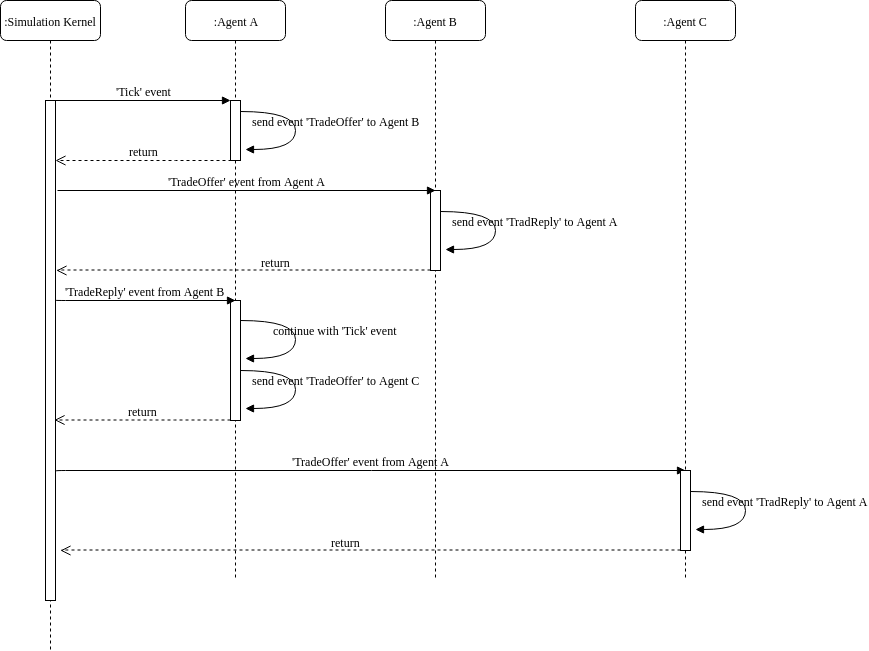
\includegraphics[width=1.0\textwidth, angle=0]{./fig/eventdriven/syncagentinteractions.png}
	\caption{Sequence diagram of synchronous agent-interaction with the trading use-case. Upon the handling of the 'Tick' event, Agent A looks for trading partners and finds Agent B within its neighbourhood and sends a 'TradingOffer' message. Agent B replies to this message and Agent A continues with the trading algorithm by picking up where it has left the execution when sending the message to Agent B. After Agent A has finished the trading with Agent B, it turns to Agent C, where the same procedure follows and is thus not included fully in this diagram.}
	\label{fig:syncagentinteractions}
\end{figure}

The way to implement this is to allow an agent to be able to change its internal event-handling state: to switch into different event-handlers, after having sent an event, to be able to react to the incoming reply in a specific way by encapsulating local state for the current synchronous interaction through closures and currying. Further by making use of continuations the agent can pick up the processing of the 'Tick' event after the synchronous agent-interaction has finished. Key to this is the function \textit{continueWithAfter} which we already shortly introduced through \textit{generalEventHandler}. This function takes an MSF which returns an output b and an optional MSF. If this optional Maybe MSF is Just then the \textit{next} input is handled by this new MSF. In case no new MSF is returned (Nothing), the MSF will stay the same. This is a more specialised version of the \textit{switch} combinator introduced in Chapter \ref{sec:back_frp} in the way that it doesn't need an additional function to produce the actual MSF continuation. Note that the semantics are different though: whereas \textit{continueWithAfter} only applies the new MSF in the \textit{next} step, \textit{switch} runs the new MSF immediately. The implementation of the function is as follows:

\begin{HaskellCode}
continueWithAfter :: Monad m => MSF m a (b, Maybe (MSF m a b)) -> MSF m a b
continueWithAfter msf = MSF (\a -> do
  ((b, msfCont), msf') <- unMSF msf a
  let msfNext = fromMaybe (continueWithAfter msf') msfCont
  return (b, msfNext))
\end{HaskellCode}

We can now look at the Tick handling function. It returns a Maybe (EventHandler g) which if is Just will result in to a change of the top-level event handler through \textit{continueWithAfter} as shown in \textit{generalEventHandler} above. Note the use of continuations in the case of \textit{agentMating, agentTrade, agentLoan}. All these functions return a Maybe (EventHandler g) because all of them can potentially result in synchronous agent-interactions which require to change the top-level event handler. When calling \textit{agentDisease} we are passing a default continuation which simply switches back into \textit{generalEventHandler} to finish the processing of a Tick in an agent.

\begin{HaskellCode}
handleTick :: RandomGen g => DTime -> AgentLocalMonad g (Maybe (EventHandler g))
handleTick dt = do
  agentAgeing dt
  
  harvestAmount <- agentMove
  metabAmount   <- agentMetabolism
  agentPolute harvestAmount metabAmount

  ifThenElseM
    (starvedToDeath `orM` dieOfAge)
    (do
      agentDies agentMsf
      return Nothing) 
    -- pass agentContAfterMating as continuation to pick up after mating
    -- synchronous conversations have finished
    (agentMating agentMsf agentContAfterMating)

-- after mating continue with cultural process and trading
agentContAfterMating :: RandomGen g => AgentLocalMonad g (Maybe (EventHandler g))
agentContAfterMating = do
    agentCultureProcess
    -- pass agentContAfterTrading as continuation to pick up after trading 
    -- synchronous conversations have finished
    agentTrade agentContAfterTrading 

-- after trading continue with lending and borrowing
agentContAfterTrading :: RandomGen g  => AgentLocalMonad g (Maybe (EventHandler g))
agentContAfterTrading = agentLoan agentContAfterLoan

-- after lending continue with diseases, which is the step in a Tick event
agentContAfterLoan :: RandomGen g => AgentLocalMonad g (Maybe (EventHandler g))
agentContAfterLoan = agentDisease defaultCont

-- safter diseases imply switch back into the general event handler
defaultCont :: RandomGen g => AgentLocalMonad g (Maybe (EventHandler g))
defaultCont = return (Just generalEventHandler)
\end{HaskellCode}

\subsection{Environment Representation}
Environment representation is quite simpl, after we have solved the problem of how the agent can access it by using StateT. It is only a matter of selecting the right data-structure and writing domain-specific functions of the corresponding model to mutate the environment. Initially we used an indexed array from the \textit{array} package. This data-structure has excellent read performance but in performance tests it was shown that it has serious performance and memory leak issues with updates, leading to allocation of about 40 MByte / second on our machine. Clearly this is unacceptable for simulation purposes, which often requires software to run for hours, and thus needs a constant memory consumption and must prevent even slowly linearly increasing memory usage under all costs. The solution was to switch to \textit{IntMap} from the \textit{containers} package as an underlying data-structure. We used the discrete 2d-coordinates to map the environment cells to a unique index. This solved both the performance and memory leak issues completely.

\subsubsection{Environment Behaviour}
We must make a clear distinction between the environments data-structure and how agents access it and the environments behaviour. In the Sugarscape model, the behaviour of the environment is quite trivial: it simply regrows resources over time and diffuses pollution in case pollution is turned on. This behaviour is achieved by providing a pure function without any monadic context or MSF. This is not necessary because the environment how we implement it, does not encapsulate local state and it does not interact with agents through messages and vice versa. Thus a pure function which maps the environment to the environment is enough: \textit{Time $\rightarrow$ SugEnvironment $\rightarrow$ SugEnvironment}. Further it also takes the current simulation time so it can implement seasons, where the speed of regrowth of resources is different in different regions and swaps after some time. This function is called in the simulation kernel after every Tick (see below).

Generally, one can distinguish between four different types of environments in ABS:

\begin{enumerate}
	\item \textit{Passive read-only} - implemented in Chapter \ref{sec:timedriven_firststep}, where the environment itself is not modelled as an active process and is static information, e.g. a list of neighbours, passed to each agent. The agents cannot change the environment actively - in the case of Chapter \ref{sec:timedriven_firststep} this is enforced at compile time by simply excluding it from the data an agent can emit. Note the agents change the environment implicitly by changing their state but there is no notion of an active environment process.
	
	\item \textit{Passive read/write} - implemented in Chapter \ref{sec:adding_env}. The environment is just shared data, which can be accessed and manipulated by the agents. Note that this forces some arbitration mechanism to prevent conflicting updates e.g. running the agents sequentially one after the other, to ensure that only one agent has access at a time.
	
	\item \textit{Active read/write} - as implemented above. To make it active a pure function is used where the environment data is owned by the simulation kernel and then made available to the agents through a State Monad. Another approach would be to implement the environment process as an agent, which is run together with all the other agents. This allows the environment to send and receive messages but the guarantees about when the environment will be run is lost if agents are run random sequentially.
	
	\item \textit{Active read-only} - can be implemented as above but instead of providing the environment data through a State Monad, a Reader Monad is used. The environment data is owned by the Simulation kernel and the process runs as a pure function as before but the data is provided in a read-only way through the Reader Monad.
\end{enumerate}

\subsection{The simulation kernel}
The simulation kernel is the heart of the simulation mechanism: it holds the full simulation state and iterates the simulation step-by-step through virtual time. The full simulation state is comprised of the following: 

\begin{itemize}
	\item A mapping of agent MSFs to their id.
	\item A list of the current observable state of each agent.
	\item The state of the environment.
	\item A random-number generator.
	\item A step counter.
\end{itemize}

In each step the simulation state is used to compute the next step of the simulation and is thus updated after a state has been computed. Using pure functional programming, where we have persistent data-structures and immutable data, we can easily keep record of the simulation state for each step for debugging purposes e.g. instead of overwriting the state after each step, we can keep the state of each step and can go backwards and forwards in the time-series of steps.

The very heart of the simulation kernel is the step function, which computes the next step of the simulation. It is a \textit{pure} function, taking the current simulation state and returns a new simulation state together with the output of the new step. The output of a step is the current simulation time, the number of events processed, the environment state and a list of the observable states of all agents.

\begin{HaskellCode}
type SimStepOut = (Time, Int, SugEnvironment, [AgentObservable SugAgentObservable])
-- Need RandomGen g because holding a random-number generator in SimulationState
simulationStep :: RandomGen g => SimulationState g -> (SimulationState g, SimStepOut)
\end{HaskellCode}

The working horse behind \textit{simulationStep} is another \textit{pure} function which processes all events scheduled in the current step. It takes the list of events to process and the simulation state and returns the simulation state.

\begin{HaskellCode}
type EventList  = [(AgentId, ABSEvent SugEvent)]  -- from, to, event
processEvents :: RandomGen g => EventList -> SimulationState g -> SimulationState g
\end{HaskellCode}

To void getting too technical and mixed up in implementation details, we provide the internals of \textit{processEvents} in terms of steps done instead of code. The function does the following:

\begin{enumerate}
	\item Extract the event at the front of the \textit{EventList}. In case the list is empty, return the simulation state.
	\item Look up the receivers' agent MSF in the agent mapping of the simulation state.
	\item If the receiver was not found, the function ignores this and processes the next event through a recursive call.
	\item If the receiver is found: run the agents' MSF and get the result.
	\item Update the agents' current MSF in the mapping (note that an MSF produces a new MSF as a result!).
	\item Update the agents' current observable state.
	\item Handle the agents' output: create new agents and remove the agent from the simulation if it killed itself.
	\item Prepend the events the agent has emitted through its output to the front \textit{EventList} and do a recursive call to \textit{processEvents}.
\end{enumerate}

The initial \textit{EventList} passed to \textit{processEvents} is a list with \textit{Tick} events scheduled for every agent, in random order. It is very important to understand that the events an agent emits, are prepended to the front of the \textit{EventList}. This ensures that those events are processed next, which is of utmost importance for a correct working of the synchronous agent-interactions. This also implies that \textit{processEvents} is a potentially non-terminating function, in case there is at least one agent which produces at least one event for every event it receives.

Finally we have a look at how to actually run an agents' MSF using the function \textit{runAgentSF}. It is a \textit{pure} function as well and thus takes all input as explicit arguments. It might look like an overkill to pass in 5 arguments and get a 6-tuple as result but this is the price we have to pay for pure functional programming: everything is explicit, with all its benefits and drawbacks.

\begin{HaskellCode}
runAgentSF :: RandomGen g        -- ^ RandomGen typeclass, g is a random-number generator
           => SugAgentMSF g      -- ^ The agents MSF to run.
           -> ABSEvent SugEvent  -- ^ The event it receives.
           -> ABSState           -- ^ The ABSState (next agent id and current time)
           -> SugEnvironment     -- ^ The environment state
           -> g                  -- ^ The random-number generator
           -> (SugAgentOut g, SugAgentObservable, SugAgentMSF g, ABSState, SugEnvironment, g)
runAgentSF msf evt absState env g = (ao, obs, msf', absState', env', g') 
  where
    -- extract the monadic function to run
    msfAbsState = unMSF msf evt
    -- peel away one State layer: ABSState
    msfEnvState = runStateT msfAbsState absState
    -- peel away the second State layer: SugEnvironment
    msfRand     = runStateT msfEnvState env
    -- peel away the 3rd and last layer: Rand Monad
    (((((ao, obs), msf'), absState'), env'), g') = runRand msfRand g
\end{HaskellCode}

Note that we run only the 3 \textit{global} monadic layers in here, the 3 \textit{local} layers are indeed completely local to the agent itself as shown above.